

\chapter{Techniques for Improving Learning Models} 

\section{Capacity, Overfitting, Underfitting}
Recall, the learning algorithm (Experience, Training, Program):
The program is "trained" using Experience, as in ($x^{{(train)}},y^{{(train)}}$).
But P is determined by "test" data not found in the Experience, as in ($x^{{(test)}},y^{{(test)}}$).

Usually there will be some "cost function" which can be minimized with respect to the training set in order to determine Program. That is, the "test error" is minimized by minimizing the "training error."

In order to ensure the above process works properly, assumptions need to be made. These will be referred to as the Independent Identically Distributed (IID) assumptions. Both the training set and the test set are gotten by independently (or randomly) sampling the same probability distribution. We will refer to this probability distribution as "Pdata".

Usually our task T is accomplished by choosing some set $\overrightarrow{w}$ of parameters found by minimizing some cost function $J(\overrightarrow{w}$) on the training set.

We measure the performance of the program by measuring our cost over some training set $E^{{(train)}}$.
The process for this follows a general formula:
\begin{enumerate}
    \item Randomly sample $P_{data}$ to get $E^{{(train)}}$
    \item Find $\vw^{\ast}=\underset{\vw}{\argmin}[J(\vw;E^{{(train)}})]$
    \item Sample $P_{data}$ to get $E^{{(test)}}$
    \item Compute $J(\vw^{\ast};E^{{(test)}})$
\end{enumerate}
from this, we have that 
\begin{align*}
E_{P_{data}}[J(\vw^{\ast};E^{{(test)}}] &\geq E_{P_{data}}[\underset{\vw}{\min}J(\vw;E^{{(test)}})] \\
&=E_{P_{data}}[\underset{\vw}{\min}J(\vw;E^{{(train)}})] & \text{ by IID}\\
&=E_{P_{data}}[J(\vw^{\ast};E^{{(train)}})]
\end{align*}
So the value of our test error for a model is expected to be larger than the training error. Thus the performance of our model depends on
\begin{enumerate}
    \item Minimizing the training error
    \item Minimizing the gap between training error and test error
\end{enumerate}

If the model struggles with minimzing the training error, we refer to this as a problem of "underfitting", if the model struggles with minimizing the gap, we refer to this as a problem of "overfitting".

\subsection{The Capacity}

We now will provide an informal sense of the capacity of a learning algorithm

\begin{definition}
    The capacity of a learning algorithm is the "size" of the space of functions the algorithm can fit.
    We refer to the space of functions the algorithm can fit as the hypothesis space.
\end{definition}

\begin{remark}
    In order to more formally definite the capacity we need statistical learning theory which is outside the scope of this book.
\end{remark}

\begin{example}
    Consider linear regression with 1 variable. We have two cases
    \begin{enumerate}
        \item There are no polynomial terms. In this case, we predict with $f(x)=wx+b$. We refer to $f(x)$ as the hypothesis function. For this case, the capacity of all such functions had dimension 2.
        \item There are polynomial terms. For this specific example consider polynomial terms up to degree 4. We predict with $f(x)=w_4x^4+w_3x^3+w_2x^2+w_1x+b$. Now the capacity of our model is 5.
    \end{enumerate}
\end{example}

Suppose our dataset looks like
\begin{center}
    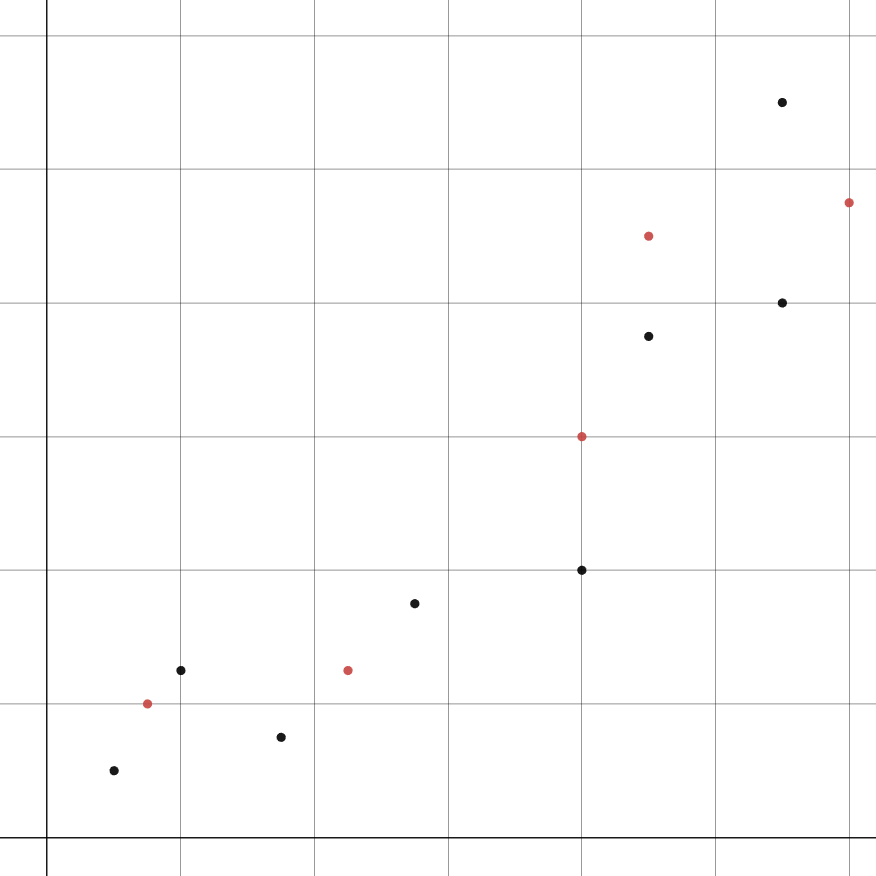
\includegraphics[width=4in]{images/Chapter7/Chapter 7 dataset.png}
\end{center}
With the black dots being our training data and the red dots being our test data. The graph of training and test error versus capacity will look something like
\begin{center}
    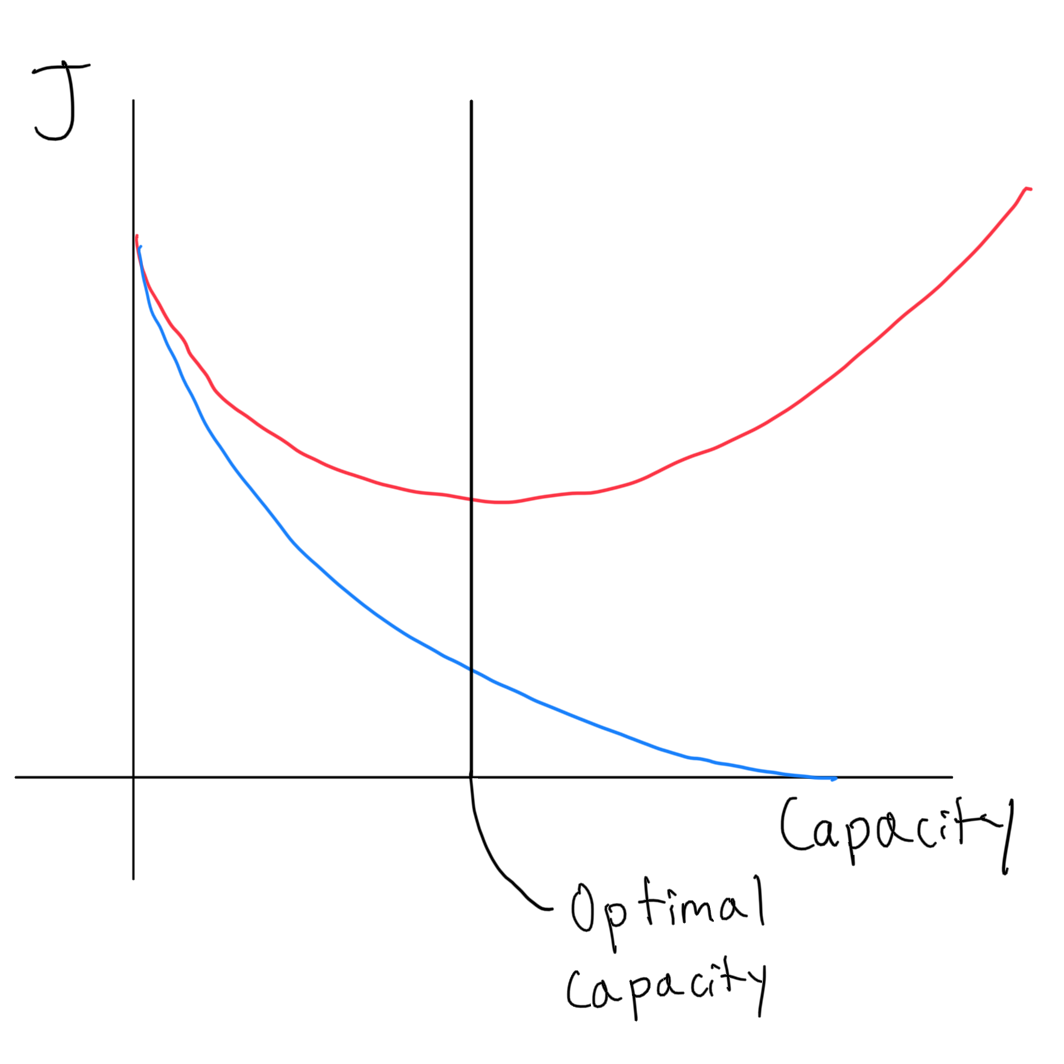
\includegraphics[width=4in]{images/Chapter7/Training vs Test Error.png}
\end{center}
with the red line representing test error and the blue line representing training error.

As you can see, there is some optimal capacity for the program in order to minimize the test error. We will further develop this "optimal model" in the next section.

\subsection{Bayes Error}

Suppose that we have $P_{data}$. We want to use $P_{data}$ to make predictions
\begin{example}
    $f^B(\vx)=\underset{y}{\argmax}P_{data}(y|\vx)$ (supervised algo)
\end{example}

Such a model will provide a theoretical minimum cost for any prediction model.

\begin{definition}
    We define Bayes Error to be $\underset{f}{\min}E_{P_{data}}[J(f;\vx, y)]$ where $J(f;\vx, y)$ is the cost function of prediction for $f(\vx)=y$.
\end{definition}

Thus the Bayes error is the error from the "optimal model" stated above.

An important note is that Bayes Error can be nonzero. For example, mapping $\vx$ to y can be nondeterministic or $\vx$ can be mapped to y in a deterministic way but it requires more variables than we have in $\MX$

\subsection{Regularization}

The central idea behind regularization is to add a new term with parameter $\lambda$ to the cost function J to further restrict the hypothesis space.

\begin{example}
    We modify $J(\vw)=\frac{1}{m}\norm{\hat{\MX}\vw-y}_2^2+\lambda\norm{\vw}_2^2$. Since we minimized J to find $\vw^\ast$, this extra term promotes coefficients of $\vw^\ast$ to be small. $\lambda$ dictates how strongly this is promoted.
\end{example}

\begin{example}
    Using polynomial terms up to degree 10
    \begin{center}
        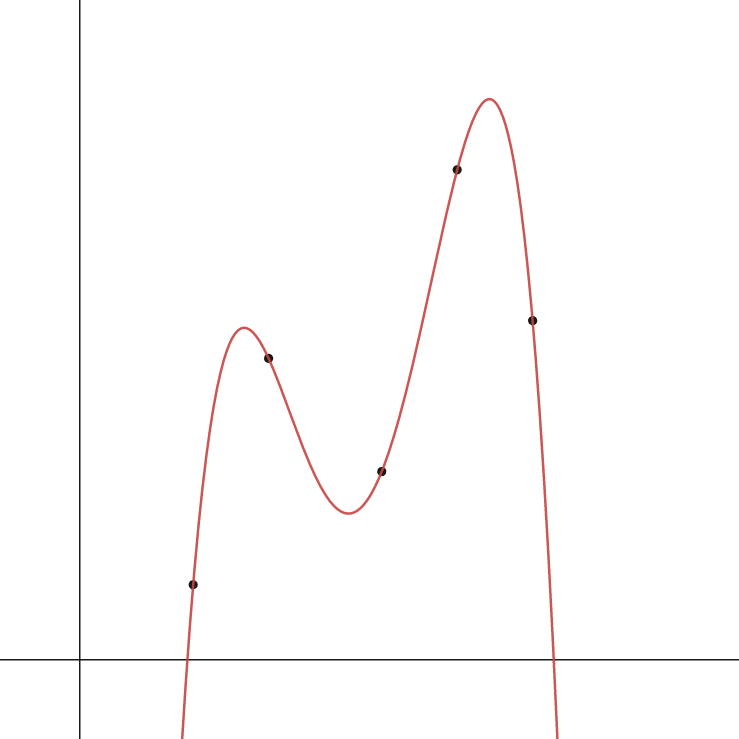
\includegraphics[width=1.75in]{images/Chapter7/Overfit.png}
        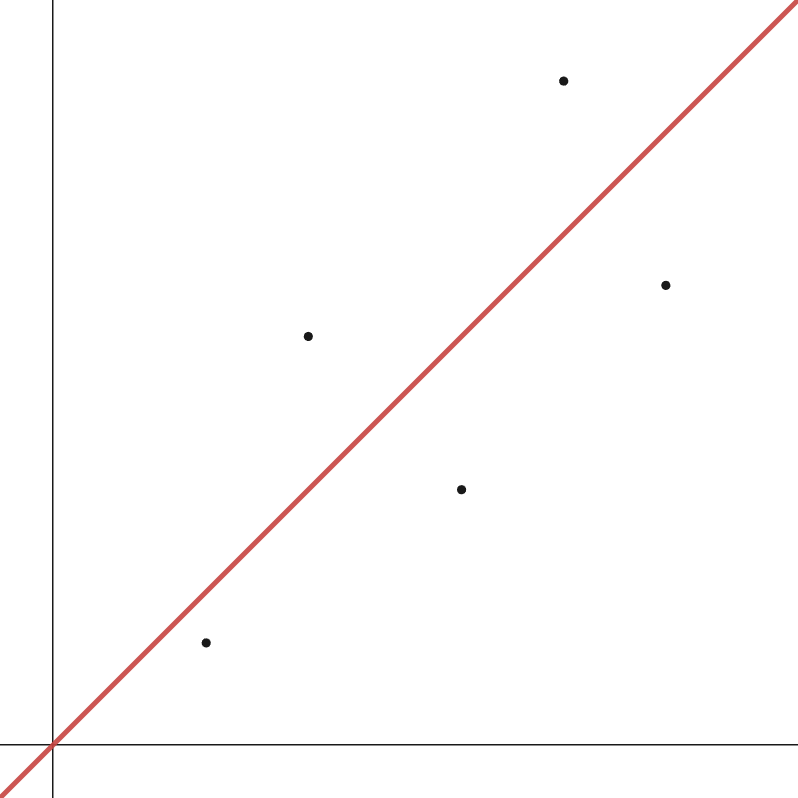
\includegraphics[width=1.75in]{images/Chapter7/Good Fit.png}
        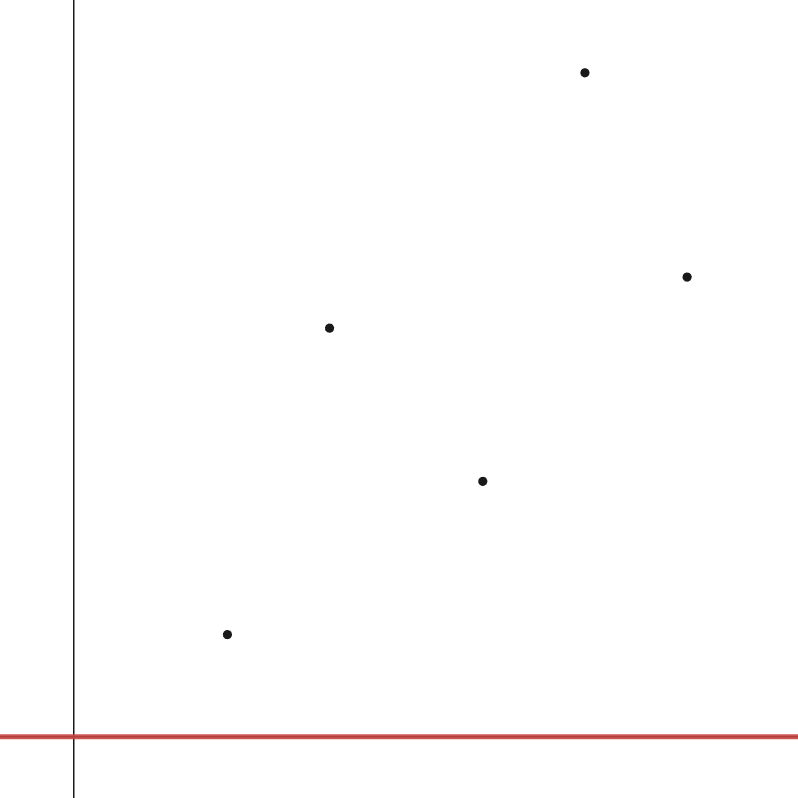
\includegraphics[width=1.75in]{images/Chapter7/Underfit.png}
    \end{center}
    The first graph has $\lambda=0$ and is overfit. The third graph has a large $\lambda$ and is underfit. The middle graph has a $\lambda$ somewhere in between and is a good fit.
\end{example}

Using regularization we can start with a high-capacity model and "tune" $\lambda$ to avoid overfitting or underfitting the data.

\section{Hyperparameters and Validation}

In the last section when we were doing regularization we added a new parameter $\lambda$. This is an example of what we call a hyperparamter.

\begin{definition}
    \define{Hyperparamters} are parameters which effect/control a learning algorithm's behaviour but are not themselves learned by the algorithm  in training.
\end{definition}

So in the aforementioned regularization example for linear regression, when we added $\lambda$ we were still minimizing the cost function over the parameter $w$ and just tuning $\lambda$ by hand.

\begin{example}
    
    In polynomial regression with regularization, the parameters are
    \[n \text{ and } \lambda \]
    where $n$ is the maximum degree of the polynomial terms (an explicit control of capacity) and $\lambda$ is the regularization parameter.
\end{example}

\subsection{A Problem:}
Hyperparameters are usually tuned by hand when experimenting in order to minimize the test error. But this creates an issue: the test set is no longer a true test set, because some model parameters are fit to the test set. And the whole point of the teat set is to approximate the generalization error, i.e. how will the model perform on new data we have never seen before. 
\subsection{A Solution and new approach:}
Introduce a new test set, which we call the validation set.
\begin{definition}
    \define{Training, validation, and test data set method}: Split the data $E$ into 3 classes, $E^{({train)}}$, $E^{{(val)}}$, and $E^{{(test)}}$. In terms of percentages, as a rule of thumb this is often a $80-10-10$ training-validation-test split.
\end{definition}

\begin{enumerate}
    \item Assuming we are trying to fit some parameters in order to create a prediction model, given hyperparameters $\vlambda$, we can train a model with $E^{{(train)}}$ by finding $\vw^{*}_{\vlambda} = \argmin_{\vw^{*}} J (\vw^{*}, \vlambda; E^{{(train)}})$.
    \item Evaluate performance on the validation dataset by looking at $J(\vw_{\vlambda}^{*} ; E^{{(val)}})$. Note that $J$ does not include the regularization term.\footnote{This is because regularization is only used during the training phase to restrict the capacity in some way, and would throw off any evaluation of performance once the parameters have already been chosen. That is, the loss function during regularization tries to penalize over/under-fitting, but once we are evaluating on a different dataset, calculating the normal loss is a much better approximation of generalization error. }
    \item Repeat 1. and 2. with different choices of $\vlambda$ until you find the lowest value of $J(\vw_{\vlambda^{*}}^{*} ; E^{{(val)}})$. Call the resulting optimal hyperparameter values $\vlambda^{*}$. This is the hyperparameter tuning phase.
    \item Approximate the generalization error by computing $J(\vw_{\vlambda^{*}}^{*} ; E^{{(test)}})$.
\end{enumerate}

\textbf{Tip:} This all works if $E$ is large enough to be split into 3 categories. If not, one possible solution is k-fold cross validation. This allows you to perform validation with your training set. In the python package sklearn, this is done with 


\begin{verbatim}
    cross_val_score()
\end{verbatim}

\section{Bias and Variance}

\begin{definition}
    A \define{point estimator} for a parameter $\theta$ associated to some distribution $p$ is any function of random variables $x_{1}, \ldots, x_{n}$ (distributed by p). We write
    \[\thetahat = y(x_{1}, \ldots, x_{n} ) \]
    The \define{bias} of $\thetahat$ is
    \[bias(\thetahat) = \Ev\left[\thetahat\right] - \theta\]
    The variance of $\thetahat$ is 
    \[Var(\thetahat) = \Ev \left[(\thetahat - \Ev \left[ \thetahat \right])^{2} \right] \]
\end{definition}

\begin{definition}
    For a given estimator, if $bias(\thetahat) = 0$ we call $\thetahat$ an \define{unbiased estimator}.
\end{definition}

\begin{example}
    Take $X_{1}, \ldots X_{n}$ IID random variables distributed by the Bernoulli Distribution:
    \[\Omega = {0, 1} \]
    \[\CP(x = 1) = \theta \]
    \[\CP(x = \chi) = \theta^{\chi}(1 - \theta)^{(1 - \chi)} \]
    
    We can make a point estimate for $\theta$ by
    \[\thetahat = \frac{\sum_{i=1}^{n} x_{i}}{n}\]
    
    Hence, our bias will be:
    \[bias(\thetahat) = \Ev\left[\thetahat\right] - \thetahat  \]
    \[= \Ev\left[ \frac{\sum_{i=1}^{n} x_{i}}{n} \right] - \thetahat\]
    and by linearity of expectation:
    \[= \frac{1}{n} \sum_{i=1}^{n} \Ev \left[x_{i}\right] - \theta \]
    \[= \frac{1}{n} \sum_{i=1}^{n} \theta - \theta \]
    \[= \frac{n\theta}{n} - \theta = 0 \]
    
    With our bias calculated, let's now look at the variance:
    \[Var(\thetahat) = Var\left( \frac{1}{n} \sum_{i=1}^{n} x_{i} \right) \]
    because $\frac{1}{n}$ is a constant, we can "bring" it's square out:
    \[= \frac{1}{n^{2}} \sum_{i=1}^{n} V(x_{i}) \]
    \[= \frac{1}{n^{2}} \sum_{i=1}^{n} \theta(1-\theta) \]
    \[= \frac{\theta(1-\theta)}{n} \]
    Notice that
    \[\lim_{n \to \infty}\frac{\theta(1-\theta)}{n} = 0 \]
    
\begin{definition}
    The \define{mean squared error} (MSE) of $\thetahat$ is
    \[MSE(\thetahat) = \Ev \left[(\thetahat - \theta)^{2} \right] \]
\end{definition}
    
\begin{lemma}
    \[MSE(\thetahat) = Var(\thetahat) + Bias(\thetahat)^{2} \]
\end{lemma}
    \begin{proof}
    \[ MSE(\thetahat) = \Ev \left[ (\thetahat - \theta)^{2} \right] \]
    \[ = \Ev \left[ (\thetahat - \Ev\left[ \thetahat \right] + \Ev\left[ \thetahat \right] - \theta)^{2}\right] \]
    \[ = \Ev \left[ (\thetahat - \Ev\left[\thetahat\right])^{2} + (\Ev\left[\thetahat\right] - \theta)^{2} + 2(\thetahat - \Ev\left[\thetahat\right])(\Ev\left[\thetahat\right] - \theta) \right] \]
    \[ = \Ev\left[ (\thetahat - \Ev\left[\thetahat\right])^{2} \right] + \Ev\left[ (\Ev \left[ \thetahat \right] - \theta)^{2} \right] + 2\Ev\left[ (\thetahat - \Ev\left[ \thetahat\right])(\Ev\left[\thetahat\right] - \theta) \right]] \]
    Note that $\Ev \left[ \thetahat \right] - \theta$ is a constant:
    \[ = Var(\thetahat) + (\Ev\left[\thetahat\right] - \theta)^{2} + 2(\Ev[\thetahat] - \theta)\Ev\left[ \thetahat - \Ev\left[\thetahat\right] \right]\]
    Notice $\Ev\left[ \thetahat - \Ev\left[\thetahat\right] \right] = \Ev\left[\thetahat\right] - \Ev\left[\thetahat\right] = 0$, so we have:
    \[= Var(\theta) + Bias(\thetahat)^{2} \]
    Which is exactly what we wanted.
    \end{proof}
    
\end{example}

Finally, it is worth pointing out that, for large data sets, it might take too much computational power to use all of it during the training process. Instead, pick a subset of the data set (mini-batch) during each iteration to approximate.


\section{Exercises}
\begin{enumerate}
    \item State the capacity for the following models:
    \begin{enumerate}
        \item Polynomial regression using terms up to the 8th degree
        \item Logistic regression using terms up to the 20th degree
        \item Linear regression using $f(x)=wx+b$
        \item Polynomial regression using $w_7x^7+w_4x^4+w_1x$
    \end{enumerate}
    \item Prove that training error can be less then Bayes error.
    \item Find the Gradient and Hessian for the new cost function after adding the regularization term, $J(\vw)=\frac{1}{m}\norm{\hat{\MX}\vw-y}_2^2+\lambda\norm{\vw}_2^2$
    \item Consider a Gaussian distribution $N(x; \mu, \sigma^{2})$. We can estimate the mean $\mu$ by taking the average of $n$ IID random variables (all from identical Gaussian distributions):
    \[\hat{\mu} = \frac{x_{1} + x_{2} + \ldots + x_{n}}{n} \]
    Show that $Bias(\hat{\mu}) = 0$.
    \item Still considering a Gaussian distribution, estimate $\sigma^{2}$ by
    \[\hat{\sigma^{2}} = \frac{1}{n} \sum_{i = 1}^{n}(x_{i} - \hat{\mu})^{2}\]
    Show that \[Bias(\hat{\sigma^{2}}) = - \frac{\sigma^{2}}{n} \]
    \item Going back to the point estimate $\hat{\mu}$ for a Gaussian distribution, find the mean squared error of $\hat{\mu}$
\end{enumerate}

\section{Solutions to Exercises}
\begin{enumerate}
    \item We have that the capacity of each of the models is:
    \begin{enumerate}
        \item 9 as there are 8 powers of x and the constant
        \item 21 as there are 20 powers of x and the constant
        \item 2 as there is just 1 power of x and the constant
        \item 3 as there are three terms total
    \end{enumerate}
    \item Here is a possible proof: Assume that you have a nondeterministic mapping of $\vx$ to y. Then Bayes error is nonzero. Consider a training set on this data. We could have a subset that can be deterministically mapped from $\vx$ to y. Thus the training error could be 0, while the Bayes error is nonzero. Thus the training error can be less than the Bayes error.
    \item In an earlier exercise we showed that the gradient of $\norm{\hat{\MX}\vw-y}_2^2=2(\hat{\MX}^\intercal\hat{\MX}\vw-\hat{\MX}^\intercal y)$ so we only have to find the gradient of $\lambda\norm{\vw}_2^2=\lambda\frac{\partial}{\partial\vw}\vw^\intercal\vw=\lambda\vw^\intercal(I+I^\intercal)=2\lambda\vw^\intercal$. Combining these gives us that the gradient is $\frac{2}{m}(\hat{\MX}^\intercal\hat{\MX}\vw-\hat{\MX}^\intercal y)+2\lambda\vw^\intercal$.\\
    To find the Hessian we take the gradient again. So we get that the Hessian is $\frac{2}{m}\hat{\MX}^\intercal\hat{\MX}+2\lambda I^\intercal=\frac{2}{m}\hat{\MX}^\intercal\hat{\MX}+2\lambda$.
    \item \[Bias(\hat{\mu}) = \Ev[\hat{\mu}] - \mu \]
    \[ = \Ev\left[\frac{x_{1} + \ldots + x_{n}}{n}\right] - \mu\]
    and then by linearity:
    \[ = \frac{\Ev[x_{1}] + \ldots + \Ev[x_{n}]}{n} - \mu\]
    \[ = \frac{\mu + \ldots + \mu}{n} - \mu\]
    \[ = \frac{n(\mu)}{n} - \mu = \mu - \mu\]
    \[ = 0\]
    So $\hat{\mu}$ is an unbiased estimator.
    \item \[Bias(\hat{\sigma^{2}}) = \Ev[\hat{\sigma^{2}}] - \sigma^{2} \]
    \[= \Ev\left[\frac{1}{n} \sum_{i = 1}^{n}(x_{i} - \hat{\mu})^{2}\right] - \sigma^{2} \]
    \[= \frac{1}{n}\sum_{i = 1}^{n}\Ev\left[x_{i}^{2} - 2x_{i}\hat{\mu}- \hat{\mu}^{2}\right]  - \sigma^{2}\]
    \[= \frac{1}{n}\sum_{i=1}^{n}(\sigma^{2} + \mu^{2}) ) \]
    \item
\end{enumerate}